\documentclass[xcolor=dvipsnames]{beamer}

\usepackage[utf8]{inputenc}
\usepackage{multicol}
\usepackage{amssymb,amsmath,amsbsy,cmath} 
\usepackage{bm}    
\usepackage{graphicx,graphics,xcolor}
\usepackage{xcolor}
\usepackage{physics}
\usepackage{comment}
\usepackage{caption}
\usepackage[style=authortitle,backend=bibtex]{biblatex}
\addbibresource{References.bib}
\usepackage{yfonts}
\usepackage{pifont}


\newcommand\blfootnote[1]{%
  \begingroup
  \renewcommand\thefootnote{}\footcite{#1}%
  \addtocounter{footnote}{-1}%
  \endgroup
}


\usetheme{Madrid}
\useoutertheme{miniframes} % Alternatively: miniframes, infolines, split
\useinnertheme{circles}


\title[Schwarzschild geometry]{Schwarzschild Geometry: Geodesics for massive particles}
\date{\today}
\author[Universidad del Valle]{Alejandro Gómez }
\institute[]{Universidad del Valle \\ Departamento de física}

\begin{document}
	
	\begin{frame}
		\titlepage
	\end{frame}
	
	\begin{frame}{Table of contents}
    \tableofcontents
	\end{frame}
	
	
\section{Generalities}

\begin{frame}{Schwarzschild metric}

Suppose a body of mass $M$. Let $\mu = GM/c^2$

$$c = 3\cdot 10^8 \text{m/s} \qquad \quad G = 6.67 \cdot 10^{-11} \text{m}^3 \text{kg}^{-1} \text{s}^{-2}$$.

\begin{block}{Line element}
\begin{equation*}
	ds^2 = c^2 \left( 1 - \frac{2\mu}{r}\right) dt^2 - \left( 1 - \frac{2\mu}{r}\right)^{-1} dr^2 - r^2 d\theta^2 - r^2 \sin^2 \theta d\phi^2
\end{equation*}
\end{block}

\begin{equation*}
    ds^2 = g_{\mu \nu} x^\mu x^\nu
\end{equation*}

\end{frame}


\begin{frame}{Geodesic equations}

The length-minimizing curves within the geometry and are given by

\begin{equation*}
    \frac{d^2 x^\mu}{d\sigma^2} + \Gamma^\mu_{\, \nu \rho} \frac{dx^\nu}{d\sigma} \frac{dx^\rho}{d\sigma} = 0
\end{equation*}

where $\sigma$ is the affine parameter.

\begin{block}{Euler-Lagrange formalism}

Equivalent form of computing the geodesics

\begin{equation*}
	\mathcal{L} \equiv g_{\mu \nu} \dot{x}^\mu \dot{x}^\nu  \longrightarrow \frac{d}{d\sigma} \left( \frac{\partial \mathcal{L}}{\partial \dot{x}^\mu} \right) - \frac{\partial \mathcal{L}}{\partial x^\mu} = 0
\end{equation*}
\end{block}

\end{frame}


\begin{frame}{Geodesic equations}

The Lagrangian is given by 

\begin{block}{}
\begin{equation*}
\mathcal{L} = c^{2}\left( 1-\frac{2\mu}{r} \right)\dot{t}^{2}-\left( 1-\frac{2\mu}{r}\right)^{-1}\dot{r}^{2}-r^{2}\left(\dot{\theta}^{2}+sen^{2}\theta\right)\dot{\phi}^{2}
\end{equation*}
\end{block}

\begin{itemize} 
    \item 4 differential equations from Euler-Lagrange equations.
    \item Variables: $x^0 = ct$, $x^1 = r$, $x^2 = \theta$, $x^3 = \phi$.
    \item $\mathcal{L}$ is cyclic on $ct$ and $\phi$
\end{itemize}

\end{frame}


\begin{frame}{Geodesic equations}
    
Confining our attention to particles moving in the equatorial plane ($\theta = \pi/2$)

\begin{itemize}
    \item $x^0 = ct$ 
    \begin{equation*}
        \left( 1 - \frac{2 \mu}{r} \right) \dot{t} = k 
    \end{equation*}
    
    \item $x^1 = r$ 
    \begin{equation*}
        \left( 1 - \frac{2 \mu}{r} \right)^{-1} \ddot{r} + \frac{2\mu}{r^2} \dot{t}^2 - \left( 1 - \frac{2 \mu}{r} \right)^{-2} \frac{\mu}{r^2} \dot{r}^2 - r\dot{\phi}^2  = 0 
    \end{equation*}
    
    \item $x^3 = \phi$ 
    \begin{equation*}
        r^2 \dot{\phi} = h
    \end{equation*}
\end{itemize}

\end{frame}



\begin{frame}{Physical interpretation of $k$ and $h$}
    
    \begin{itemize}
        \item $h = r^2 \dot{\phi}$ is the angular momentum per unit test-mass. 
        \item $k$ is related to the energy of the test-particle stored in its orbit. 
        $$k =  \left( 1 - \frac{2 \mu}{r} \right) \dot{t} = g_{00} \dot{t}$$
        $$k = g_{00} \frac{m_0 c \dot{t}}{m_0 c} = g_{00} \frac{p^0}{m_0 c}$$
        $$k = \frac{p_0}{m_0 c} = \frac{E}{m_0 c^2}$$
    \end{itemize}
    
\end{frame}



\section{Trajectories of Massive particles}


\begin{frame}{First Integral}
    
Let the proper time $\tau$ be our affine parameter, so the following holds

\begin{equation*}
    g_{\alpha \beta} \dot{x}^\alpha \dot{x}^\beta = c^2
\end{equation*}

which is equivalent to the r-equation obtained before. Thus, 
    
\begin{block}{}
\begin{eqnarray*}
\left( 1 - \frac{2 \mu}{r} \right) \dot{t} &= k \\
{\color{blue} c^2 \left( 1 - \frac{2 \mu}{r} \right) \dot{t}^2  - \left( 1 - \frac{2 \mu}{r} \right)^{-1} \dot{r}^2 - r\dot{\phi}^2 } &{\color{blue}= c^2} \\
r^2 \dot{\phi} &= h
\end{eqnarray*}
\end{block}    
\end{frame}



\begin{frame}{First Integral}
    
Using the new set of differential equations, we obtain

\begin{equation*}
\dot{r}^2 + \frac{h^2}{r^2} \left(1 - \frac{2\mu}{r} \right) - \frac{2 \mu c^2}{r} = c^2 (k^2 - 1)
\end{equation*}

Differentiating...

\begin{block}{}
\begin{equation*}
    \ddot{r} = \frac{h^2}{r^3} - \frac{3\mu h^2}{r^4} - \frac{\mu c^2}{r^2}
\end{equation*}
\end{block}

We can solve this equation and find $\phi(\tau)$ from 

\begin{equation*}
    \frac{d\phi}{d\tau} = \frac{h^2}{r^2}
\end{equation*}


\end{frame}




\begin{frame}{Trajectories}

\begin{figure}[h!]
    \centering
    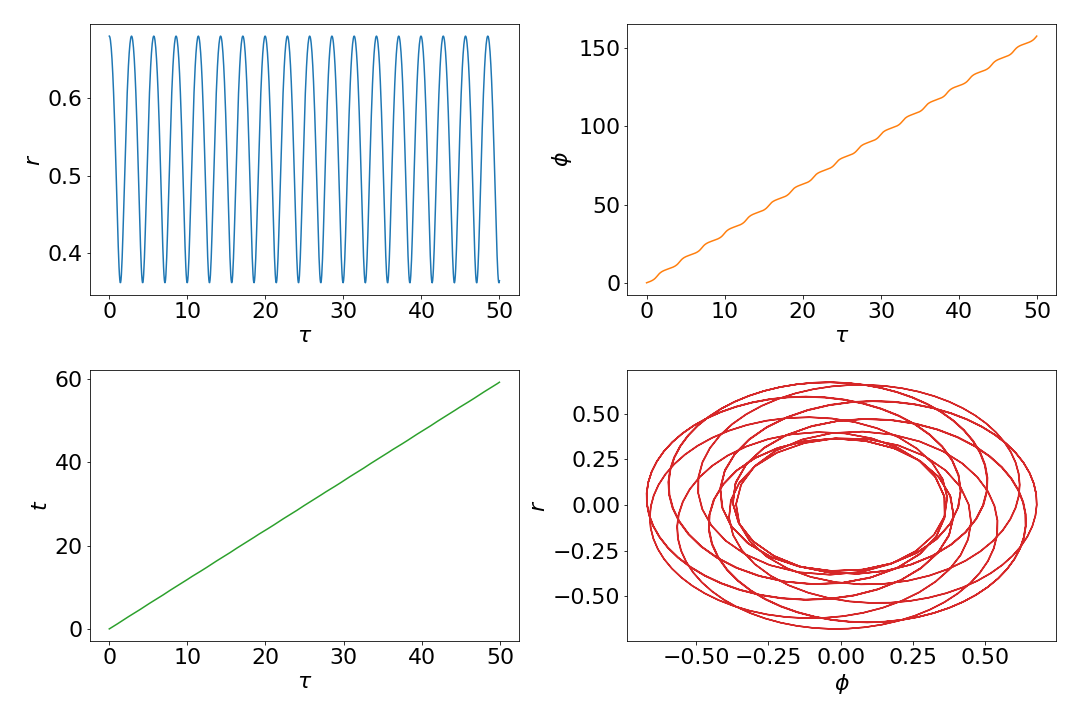
\includegraphics[width=0.8\textwidth]{Presentations/Images/2_first_orbits.png}
\end{figure}
    
\end{frame}




\begin{frame}{Trajectories}

Analogously, we could use the chain rule $\frac{dr}{d\tau} = \frac{h}{r^2} \frac{dr}{d\phi}$ and define $u = 1/r$ to convert 

\begin{equation*}
\ddot{r} = \frac{h^2}{r^3} - \frac{3\mu h^2}{r^4} - \frac{\mu c^2}{r^2}
\end{equation*}

into 

\begin{block}{}

\begin{equation*}
    \frac{d^2 u}{d\phi^2} + u = \frac{\mu c^2}{h^2} + 3 \mu u^2
\end{equation*}

\end{block}

This is a closed differential equation for the shape of the orbits.

\end{frame}




\begin{frame}{Stability}

In Newtonian mechanics, 
    
\begin{equation*}
    \frac12 \left( \frac{dr}{dt} \right)^2 + \underbrace{\frac{h^2}{2r^2} - \frac{\mu c^2}{r}}_{V_{\text{eff}}(r)} = E
\end{equation*}

whereas in Relativity,  

\begin{equation*}
    \frac12 \left( \frac{dr}{d\tau} \right)^2 + \underbrace{\frac{h^2}{2r^2} - \frac{\mu c^2}{r} - \frac{\mu h^2}{r^3}}_{V_{\text{eff}}(r)} = \frac{c^2}{2}(k^2-1)
\end{equation*}

\end{frame}



\begin{frame}{Newtonian $V_{eff}$}
    
    \begin{figure}[h!]
        \centering
        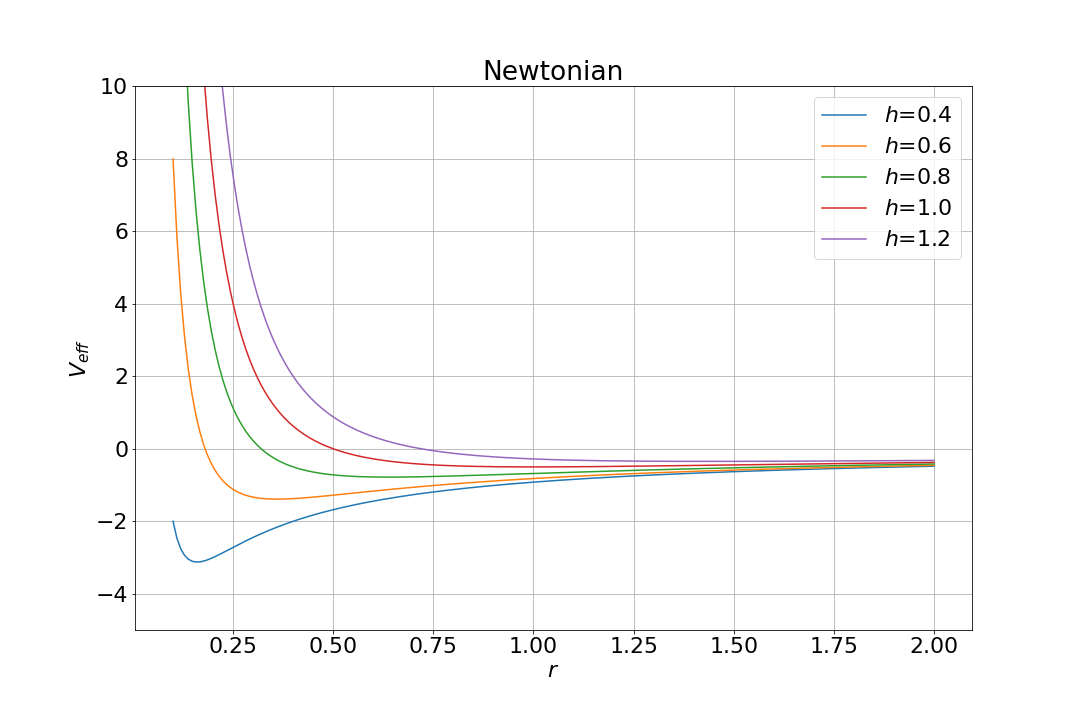
\includegraphics[width=0.8\textwidth]{Presentations/Images/2_veff_newton.png}
    \end{figure}
    
\end{frame}



\begin{frame}{Relativistic $V_{eff}$}
    
    \begin{figure}[h!]
        \centering
        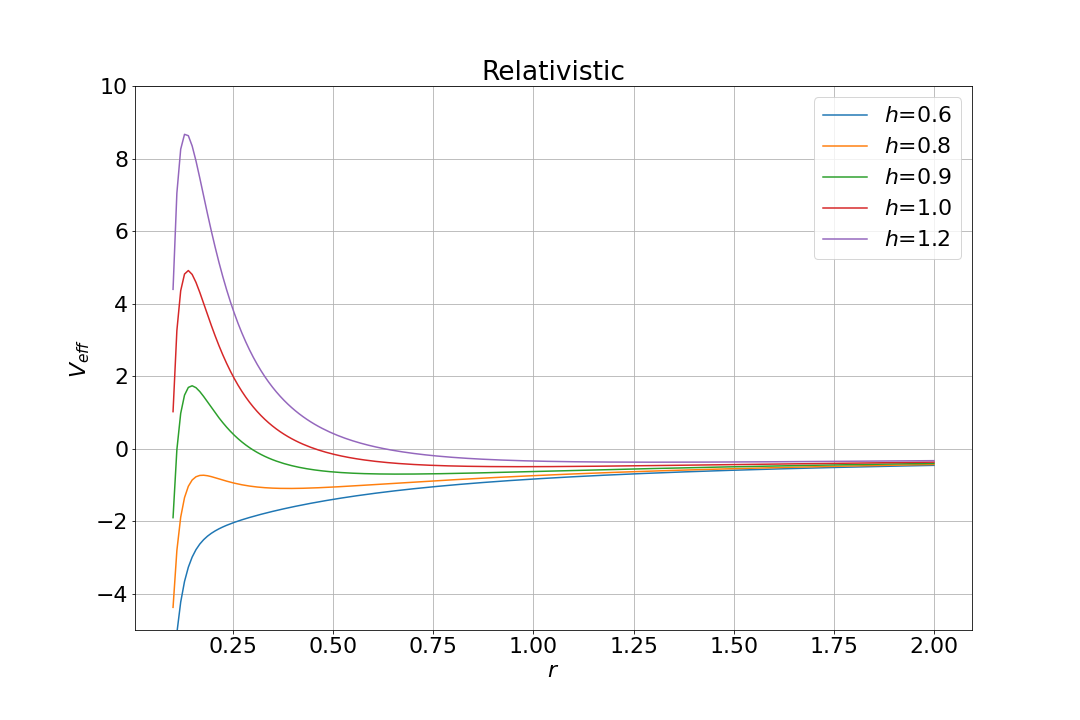
\includegraphics[width=0.8\textwidth]{Presentations/Images/2_veff_relat.png}
    \end{figure}
    
\end{frame}


\begin{frame}{Relativistic $V_{eff}$}
    
\begin{equation*}
    \left. \frac{dV_{eff}}{dr}\right|_{r=r^*} = 0 
\end{equation*}

leads us to 

\begin{block}{}

\begin{equation*}
    r^* = \frac{h}{2\mu c^2} \left( h \pm \sqrt{h^2 - 12 \mu^2 c^2} \right)
\end{equation*}

\end{block}

We have a stable (+) and unstable (-) circular orbits. 

If $h = 2\sqrt{3} \mu c$ there exists only one stable orbit with $r^* = 6 \mu$

\end{frame}


\begin{frame}{Classical and Relativistic}
    
    \begin{figure}[h!]
        \centering
        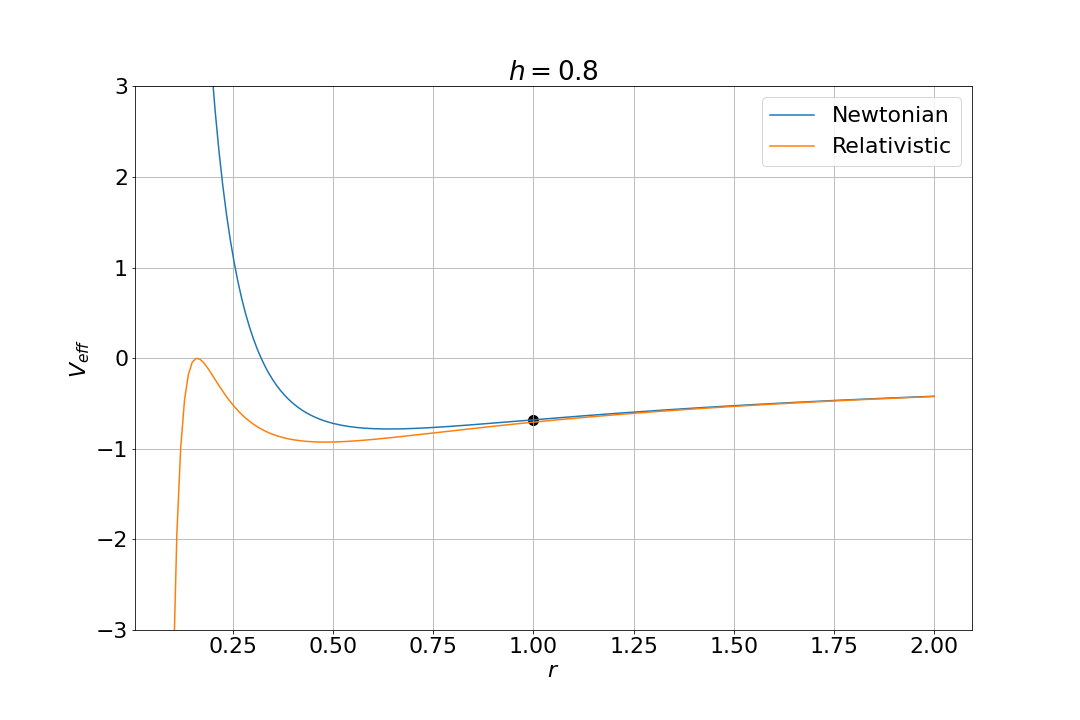
\includegraphics[width=0.8\textwidth]{Presentations/Images/2_veff_newrel.png}
    \end{figure}
    
\end{frame}



\begin{frame}{Classical and Relativistic}

        \begin{figure}[h!]
        \centering
        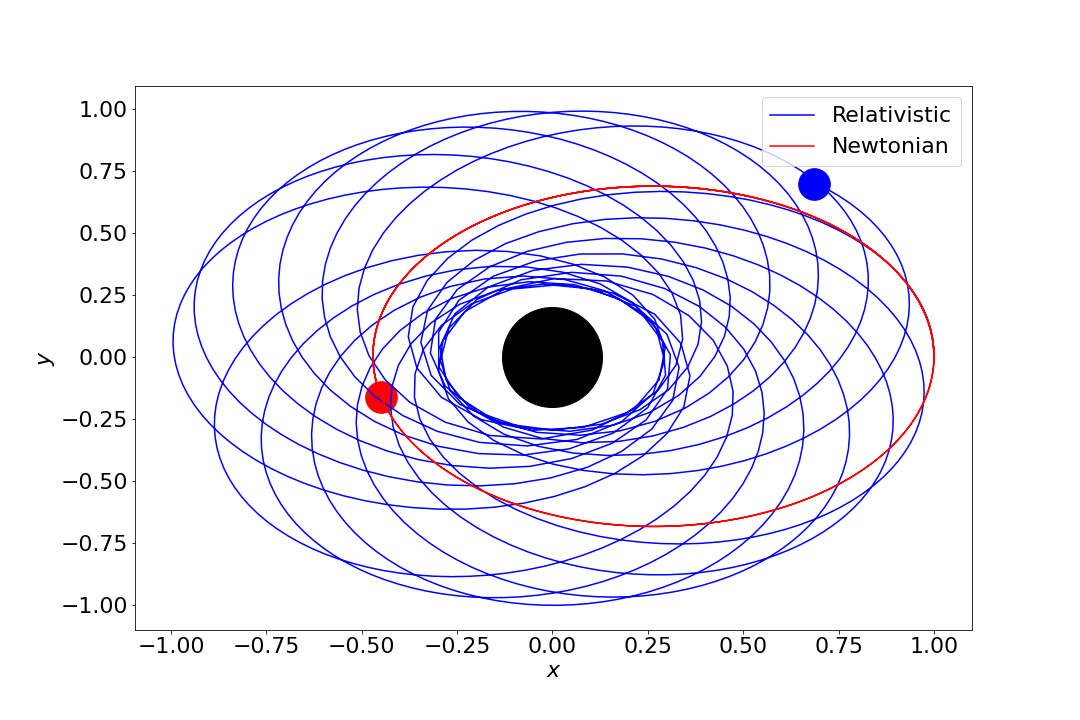
\includegraphics[width=0.8\textwidth]{Presentations/Images/2_class_rel_orbit.png}
    \end{figure}
    
\end{frame}


\section{Particular cases}


\begin{frame}{Radial motion}
    
There is no angular momentum, so $h=0$

\begin{equation*}
     \ddot{r} = \frac{h^2}{r^3} - \frac{3\mu h^2}{r^4} - \frac{\mu c^2}{r^2}
\end{equation*}
    
becomes 

\begin{block}{}
\begin{equation*}
     \ddot{r} = - \frac{GM}{r^2}
\end{equation*}
\end{block}

which has the same form of the classical solution. They are not the same, though.

\end{frame}



\begin{frame}{Circular motion}
    
There is no radial momentum, so $\dot{r}=0$

\begin{equation*}
    \frac{d^2 u}{d\phi^2} + u = \frac{\mu c^2}{h^2} + 3 \mu u^2
\end{equation*}
    
becomes 

\begin{equation*}
     u = \frac{\mu c^2}{h^2} + 3 \mu u^2
\end{equation*}

Then,

\begin{block}{}
\begin{equation*}
 h = \left( \frac{\mu c^2 r^2}{r - 3\mu} \right)^{1/2}
\end{equation*}
\end{block}

There exists no valid circular orbit below $r = 3\mu$. 

\end{frame}


\section{A more general case}


\begin{frame}{Out of the Equator}

If the condition $\theta = \pi/2$ is not imposed, the equations read

\begin{block}{}
\begin{align*}
\ddot{\theta} &= -\frac{2}{r} \dot{r} \dot{\theta} + \frac{\cos \theta}{r^4 \sin^3 \theta} h^2  \\
\ddot{r} &= -\frac{\mu c^2 k^2}{r^2} + \left( 1 - \frac{2\mu}{r}\right)^{-1} \frac{\mu}{r^2}\dot{r}^2 + r^2 \dot{\theta}^2 + \frac{h^2}{r^2 \sin^2 \theta} 
\end{align*}
\end{block}

which can be easily solved numerically.

\end{frame}



\begin{frame}{Outside the Equator}

\begin{figure}[h!]
   \centering
   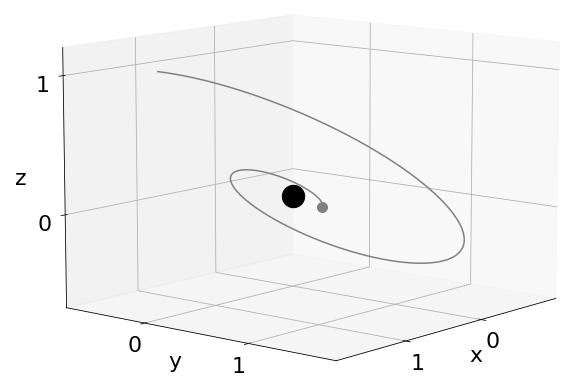
\includegraphics[width=0.75\textwidth]{Presentations/Images/2_gen_obit1.png}
\end{figure}

\end{frame}



\section{Exercises}

\begin{frame}{Problem Statements}

    \begin{block}{Conceptual}
    \begin{itemize}
        \item What happens if we add another body? Would the spherical symmetry be conserved?
    \end{itemize}
    \end{block}    
    
    \begin{block}{Analytical}
    \begin{itemize}
        \item Differentiate $g_{\alpha \beta} \dot{x}^\alpha \dot{x}^\beta = c^2$ and compare with the initial set of differential equations.
    \end{itemize}    
    \end{block}
    
    \begin{block}{Numerical}
    \begin{itemize}
        \item Obtain the graphs shown throughout this presentations and play with the parameters.
    \end{itemize}
    \end{block}
    
    \url{github.com/alejandrogm668/Schwarzschild-Geodesics.git}
    
\end{frame}


\end{document}